\documentclass[a4paper, 12pt]{article}
\usepackage[top=2cm, bottom=2cm, left=2.5cm, right=2.5cm]{geometry}
\usepackage[utf8]{inputenc}
\usepackage{amsmath, amsfonts, amssymb}
\usepackage{float}
\usepackage{graphicx}
\usepackage[brazil]{babel}
\usepackage{indentfirst} % indentação do primeiro paragráfo da seção

% Informações do trabalho
\title{TITULO DO TRABALHO}
\author{NOME DO AUTOR \\ instituição, email, etc}
\date{mês/ano}

\begin{document}
\maketitle % insere as informações do trabalho
\newpage % insere uma nova página

\tableofcontents % cria o sumário
\newpage

\listoffigures % cria a lista de figuras
\newpage

\listoftables % cria a lista de tabelas
\newpage

\section{Titulo da seção} % cria uma seção no corpo do trabalho(em 'article' temos seções, subseções e sub-subseções)

Texto texto texto texto. Texto texto texto texto. Texto texto texto texto. Texto texto texto texto.
Texto texto texto texto. Texto texto texto texto. Texto texto texto texto. Texto texto texto texto.
Texto texto texto texto. Texto texto texto texto. Texto texto texto texto. Texto texto texto texto.
Texto texto texto texto. Texto texto texto texto. Texto texto texto texto. Texto texto texto texto.
Texto texto texto texto. Texto texto texto texto. Texto texto texto texto. Texto texto texto texto.
Texto texto texto texto. Texto texto texto texto. Texto texto texto texto. Texto texto texto texto.
Texto texto texto texto. Texto texto texto texto. Texto texto texto texto. Texto texto texto texto.
Texto texto texto texto. Texto texto texto texto. Texto texto texto texto. Texto texto texto texto.
Texto texto texto texto. Texto texto texto texto. Texto texto texto texto. Texto texto texto texto.

\begin{figure}[!htb]
	\centering
	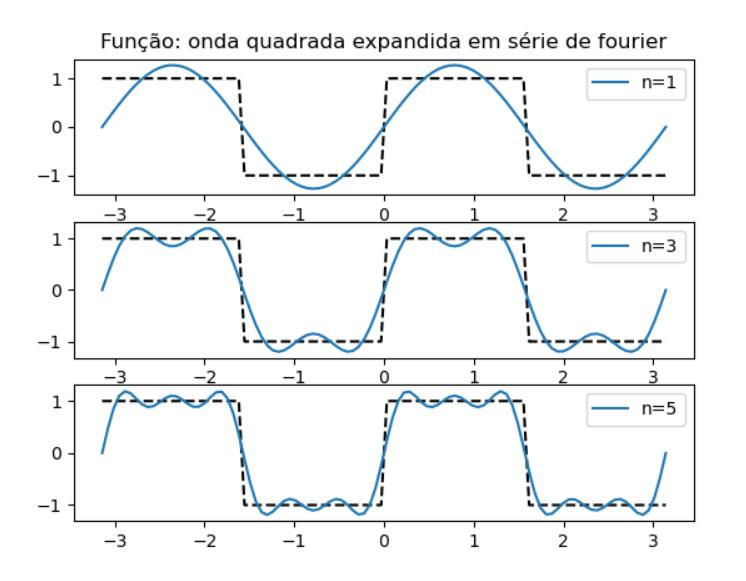
\includegraphics[scale=0.5]{img/fig1.png}
	\caption{Gráfico feito em python}
	\label{grafico-python}
\end{figure}

Texto texto texto texto. Texto texto texto texto. Texto texto texto texto. Texto texto texto texto.
Texto texto texto texto. Texto texto texto texto. Texto texto texto texto. Texto texto texto texto.
Texto texto texto texto. Texto texto texto texto. Texto texto texto texto. Texto texto texto texto.
Texto texto texto texto. Texto texto texto texto. Texto texto texto texto. Texto texto texto texto.
Texto texto texto texto. Texto texto texto texto. Texto texto texto texto. Texto texto texto texto.
Texto texto texto texto. Texto texto texto texto. Texto texto texto texto. Texto texto texto texto.
Texto texto texto texto. Texto texto texto texto. Texto texto texto texto. Texto texto texto texto.
Texto texto texto texto. Texto texto texto texto. Texto texto texto texto. Texto texto texto texto.
Texto texto texto texto. Texto texto texto texto. Texto texto texto texto. Texto texto texto texto.

\section{Titulo da seção}

Texto texto texto texto. Texto texto texto texto. Texto texto texto texto. Texto texto texto texto.
Texto texto texto texto. Texto texto texto texto. Texto texto texto texto. Texto texto texto texto.
Texto texto texto texto. Texto texto texto texto. Texto texto texto texto. Texto texto texto texto.
Texto texto texto texto. Texto texto texto texto. Texto texto texto texto. Texto texto texto texto.
Texto texto texto texto. Texto texto texto texto. Texto texto texto texto. Texto texto texto texto.
Texto texto texto texto. Texto texto texto texto. Texto texto texto texto. Texto texto texto texto.
Texto texto texto texto. Texto texto texto texto. Texto texto texto texto. Texto texto texto texto.
Texto texto texto texto. Texto texto texto texto. Texto texto texto texto. Texto texto texto texto.
Texto texto texto texto. Texto texto texto texto. Texto texto texto texto. Texto texto texto texto.

\begin{table}[htb]
	\centering
	\begin{tabular}{|c|c|}
		\hline
		$a_{0, 0}$ & $a_{0, 1}$ \\ \hline
		$a_{1, 0}$ & $a_{1, 1}$ \\ \hline
	\end{tabular}
	\caption{Um exemplo de tabela}
	\label{ex-tabela}
\end{table}

Texto texto texto texto. Texto texto texto texto. Texto texto texto texto. Texto texto texto texto.
Texto texto texto texto. Texto texto texto texto. Texto texto texto texto. Texto texto texto texto.
Texto texto texto texto. Texto texto texto texto. Texto texto texto texto. Texto texto texto texto.
Texto texto texto texto. Texto texto texto texto. Texto texto texto texto. Texto texto texto texto.
Texto texto texto texto. Texto texto texto texto. Texto texto texto texto. Texto texto texto texto.
Texto texto texto texto. Texto texto texto texto. Texto texto texto texto. Texto texto texto texto.
Texto texto texto texto. Texto texto texto texto. Texto texto texto texto. Texto texto texto texto.
Texto texto texto texto. Texto texto texto texto. Texto texto texto texto. Texto texto texto texto.
Texto texto texto texto. Texto texto texto texto. Texto texto texto texto. Texto texto texto texto.

	\subsection{Titulo da subseção}

	Texto texto texto texto. Texto texto texto texto. Texto texto texto texto. Texto texto texto texto.
	Texto texto texto texto. Texto texto texto texto. Texto texto texto texto. Texto texto texto texto.
	Texto texto texto texto. Texto texto texto texto. Texto texto texto texto. Texto texto texto texto.
	Texto texto texto texto. Texto texto texto texto. Texto texto texto texto. Texto texto texto texto.
	Texto texto texto texto. Texto texto texto texto. Texto texto texto texto. Texto texto texto texto.
	Texto texto texto texto. Texto texto texto texto. Texto texto texto texto. Texto texto texto texto.
	Texto texto texto texto. Texto texto texto texto. Texto texto texto texto. Texto texto texto texto.
	Texto texto texto texto. Texto texto texto texto. Texto texto texto texto. Texto texto texto texto.
	Texto texto texto texto. Texto texto texto texto. Texto texto texto texto. Texto texto texto texto.

		\subsubsection{Titulo da sub-subseção}

		Texto texto texto texto. Texto texto texto texto. Texto texto texto texto. Texto texto texto texto.
		Texto texto texto texto. Texto texto texto texto. Texto texto texto texto. Texto texto texto texto.
		Texto texto texto texto. Texto texto texto texto. Texto texto texto texto. Texto texto texto texto.
		Texto texto texto texto. Texto texto texto texto. Texto texto texto texto. Texto texto texto texto.
		Texto texto texto texto. Texto texto texto texto. Texto texto texto texto. Texto texto texto texto.
		Texto texto texto texto. Texto texto texto texto. Texto texto texto texto. Texto texto texto texto.
		Texto texto texto texto. Texto texto texto texto. Texto texto texto texto. Texto texto texto texto.
		Texto texto texto texto. Texto texto texto texto. Texto texto texto texto. Texto texto texto texto.
		Texto texto texto texto. Texto texto texto texto. Texto texto texto texto. Texto texto texto texto.
		
		\begin{figure}[!htb]
			\centering
			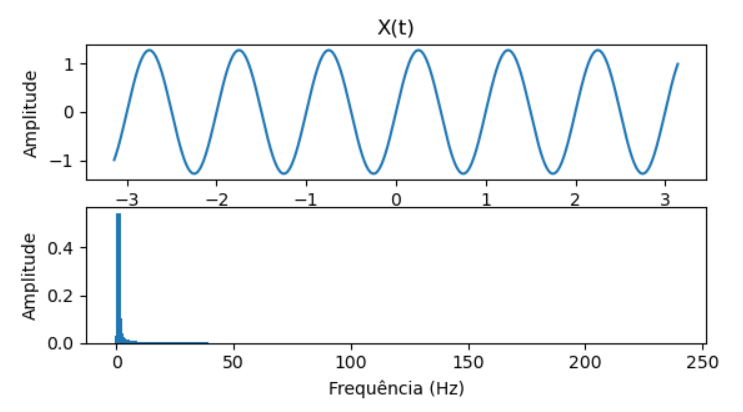
\includegraphics[scale=0.5]{img/fig2.png}
			\caption{Gráfico da frequência}
			\label{grafico-frequencia}
		\end{figure}

	\subsection{Titulo da subseção}

	Texto texto texto texto\cite{labelLivro}. Texto texto texto texto. Texto texto texto texto. Texto texto texto texto.
	Texto texto texto texto. Texto texto texto texto. Texto texto texto texto. Texto texto texto texto.
	Texto texto texto texto. Texto texto texto texto. Texto texto texto texto. Texto texto texto texto.
	Texto texto texto texto. Texto texto texto texto. Texto texto texto texto. Texto texto texto texto.
	Texto texto texto texto. Texto texto texto texto. Texto texto texto texto. Texto texto texto texto.
	Texto texto texto texto. Texto texto texto texto. Texto texto texto texto. Texto texto texto texto.
	Texto texto texto texto. Texto texto texto texto. Texto texto texto texto. Texto texto texto texto.
	Texto texto texto texto. Texto texto texto texto. Texto texto texto texto. Texto texto texto texto.
	Texto texto texto texto. Texto texto texto texto. Texto texto texto texto. Texto texto texto texto\cite{labelArtigo}.
	
	\begin{table}[htb]
		\centering
		\begin{tabular}{|c|c|}
			\hline
			$b_{0, 0}$ & $b_{0, 1}$ \\ \hline
			$b_{1, 0}$ & $b_{1, 1}$ \\ \hline
		\end{tabular}
		\caption{Outro exemplo de tabela}
		\label{ex-tabela-2}
	\end{table}

% Adicionando as referencias bibliograficas
\newpage
\bibliographystyle{plain}
\addcontentsline{toc}{section}{Referências} % inserindo a referencia no sumario
\bibliography{refs/referencias.bib}

\end{document}